\section{SDN}
\subsection{SDN의 개념}
    SDN (Software Defined Network, 소프트웨어 정의 네트워크)은 소프트웨어 프로그래밍을 통해 네트워크 경로 설정과 제어 및 복잡한 운용관리를 편리하게 처리할 수 있는 차세대 네트워킹 기술을 말한다. SDN의 핵심은 네트워크 장비의 제어부(Control Plane)와 전송부(Data Plane)의 분리이다. 제어부는 네트워크 장비를 제어하는 ‘Routing’ 역할을, 전송부는 데이터를 전송하는 ‘Forwarding’ 역할을 한다. \\
    기존의 개별 네트워크 장비는 제어부와 전송부 모두 가지고 있었다. 과거의 네트워크는 서버-클라이언트 중심 디자인이 대부분이었다. 인터넷 초창기에는 대부분의 통신이 클라이언트와 서버 간의 통신이었기 때문에 이런 단순한 구조가 문제되지 않았다. 하지만 모바일 기기가 급증하고, 클라우드 기반 가상화 서비스가 등장하면서 트래픽 패턴이 달라졌다. \\
    과거의 서버-클라이언트 통신과 달리 애플리케이션은 다수의 가상머신(Virtual Machine)에 분산되어 다양한 트래픽을 생성한다. 기업은 폭발하는 비즈니스와 사용자 요구에 맞추어 네트워크 규모를 확대하려하면서 네트워크 관리가 더욱 복잡해졌다. \\
    또, 기존의 제어부와 전송부 모두 가지고 있는 네트워크 장비는 빠르게 변화하는 네트워크 환경에 대응하기에 신속성이 부족했다. 네트워크 장비 제품의 수명주기는 3~4년에 불과했고, 표준 API나 개방된 인터페이스가 없었기 때문에 기업이 자사 네트워크 환경에 맞게 기능을 추가하는 것을 제한했다. \\
    이러한 환경 속에서 SDN이 탄생했다. SDN은 제어부를 접근 가능한 컴퓨터 장치로 분리시켜 사용자가 소프트웨어로 네트워크를 관리하고 제어할 수 있도록 만드는 기술이다. \\
    \vspace{-4mm}
    \begin{figure}[!h]\centering
		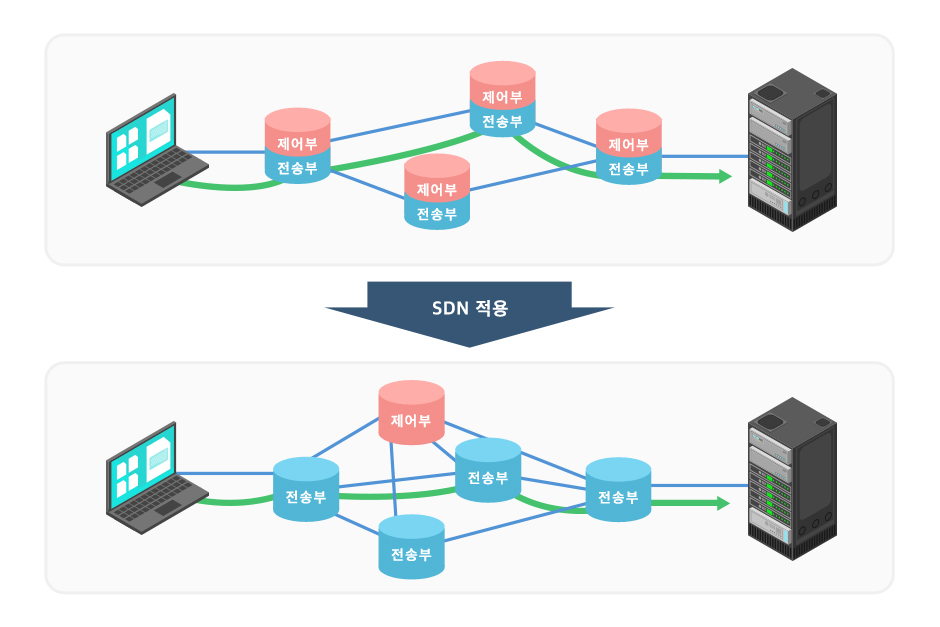
\includegraphics[width=.65\textwidth]{image/week05/1-1.png}
		\caption{\small SDN Network}
		\vspace{-10pt}
    \end{figure}
    
\subsection{SDN의 장점}
    SDN은 네트워크 가상화를 통해 제어부를 하드웨어에서 소프트웨어로 전환해 물리적 리소스 한계에 구애받지 않는다. 시시각각 변하는 네트워크 환경에 맞게 네트워크 리소스를 유연하게 확장, 축소할 수 있다. \\
    기존의 네트워크와 같이 스위치와 라우터를 개별적으로 설정할 필요 없이 사용자가 소프트웨어로 중앙화, 원격화된 네트워크를 간편하게 관리할 수 있다. \\
    기존의 제어부가 포함된 값비싼 네트워크 장비와 달리 범용 스위치, 라우터 등의 저렴한 하드웨어를 사용할 수 있다. 또한 SDN은 소프트웨어로 여러 네트워크 장비를 제어하기 때문에 기존 네트워크보다 운영 비용이 적다. \\
    
\subsection{SDN의 구성}
    \vspace{-4mm}
    \begin{figure}[!h]\centering
		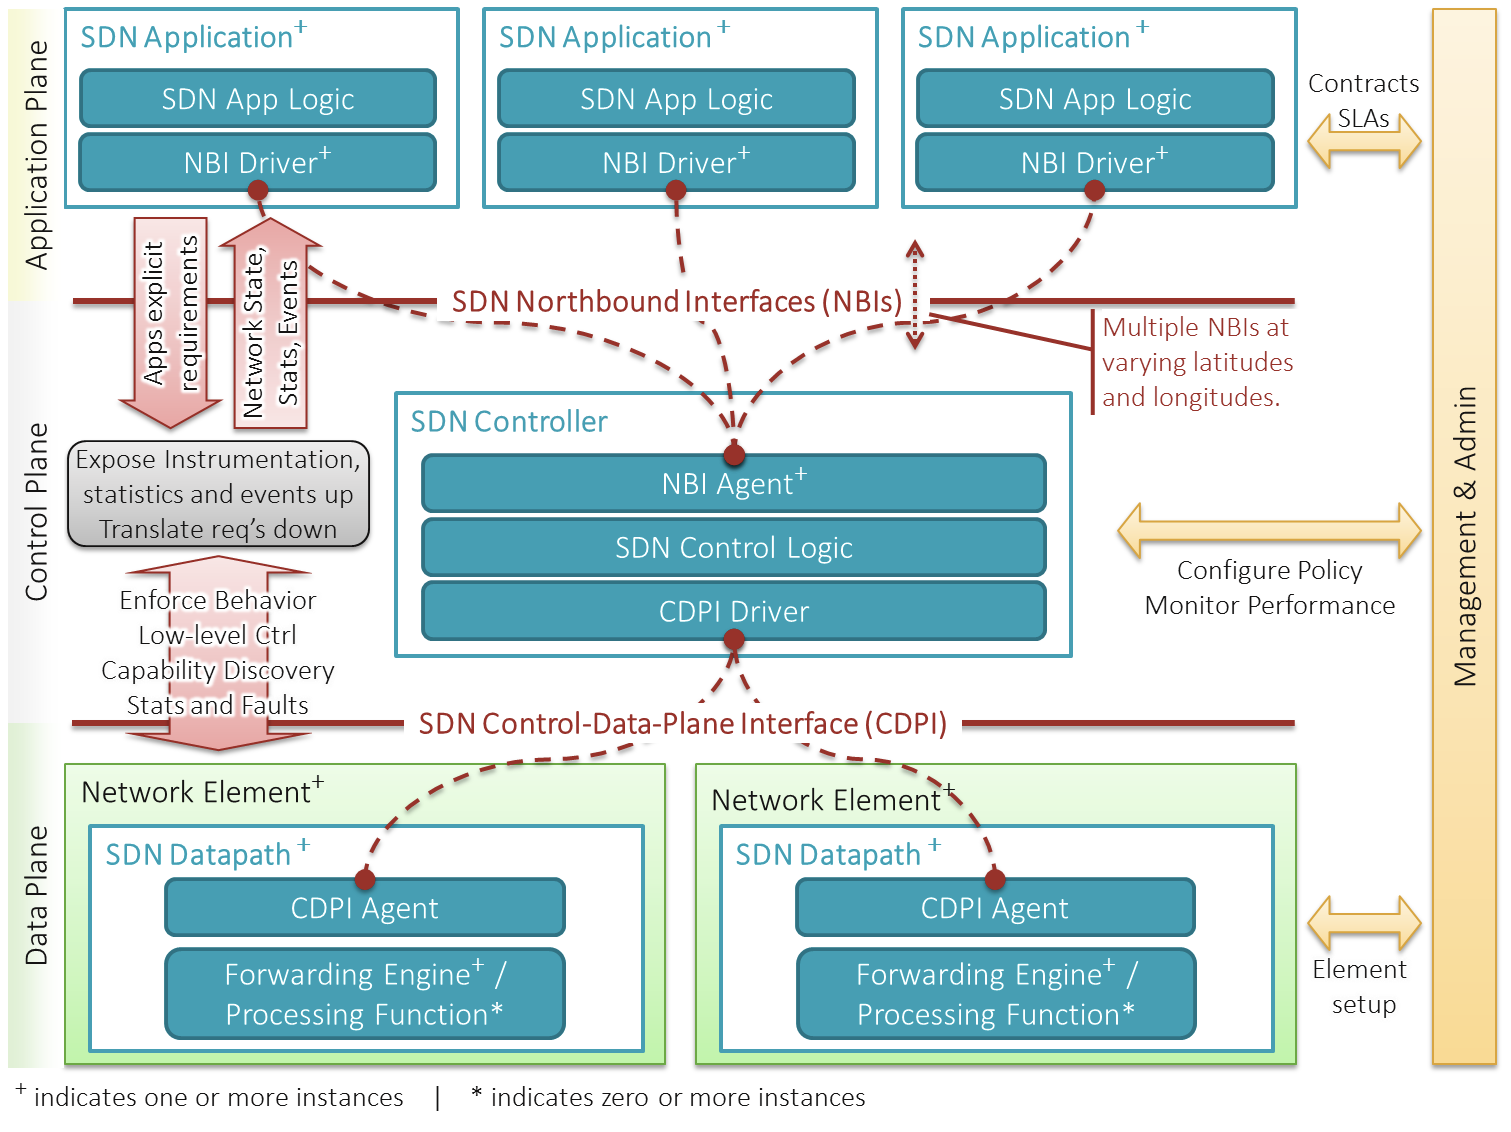
\includegraphics[width=.65\textwidth]{image/week05/1-2.png}
		\caption{\small SDN Architecture}
		\vspace{-10pt}
    \end{figure}
    SDN 아키텍처는 Application Layer, Control Plane(SDN 컨트롤러), Data Plane(SDN 전송장비) 3계층 구조이다. 각 계층 사이에는 계층 간의 연동을 위한 Southbound Interface와 Northbound Interface가 존재한다.
    
    \subsubsection*{Application Layer}
    소프트웨어 어플리케이션을 통해 사용자가 요구하는 네트워크 조건을 만족할수 있도록 Control Plane과 네트워크 관련 정보를 통신한다. \\
    
    \subsubsection*{Control Plane}
    Control Plane은 전체 네트워크 자원에 대한 중앙 집중적 제어를 담당한다. 어플리케이션 정보를 활용하여 데이터 패킷 라우팅 방식을 결정하고, 각 네트워크 장비에게 포워딩 규칙을 전달한다. 또한 여러 네트워크 장비와 통신할 수 있도록 Southbound interface를 제공하거나 추가할 수 있으며, 여러 가지 기능의 애플리케이션을 개발하고 다른 운영 도구과 통신할 수 있게 해주는 Northbound interface도 제공한다. \\
    
    \subsubsection*{Data Plane}
    Data Plane의 네트워크 장치는 Control Plane에서 정한 포워딩 규칙대로 각 데이터 패킷을 다음 장치로 수신한다. \\
\newpage